
\documentclass{sig-alternate-br}

\pagenumbering{arabic}

\usepackage{graphicx}
\graphicspath{{images/}}

\begin{document}
	
\conferenceinfo{24$^{th}$ Twente Student Conference on IT}{January 22$^{st}$, 2016, Enschede, The Netherlands.}
\CopyrightYear{2016}

\title{Low-Resource Face Spoofing Detection in a User-friendly Manner}


\numberofauthors{1}

\author{
\alignauthor
Rien Heuver\\
       \affaddr{University of Twente}\\
       \affaddr{P.O. Box 217, 7500AE Enschede}\\
       \affaddr{The Netherlands}\\
       \email{rienheuver@gmail.com}
}

\maketitle

\begin{abstract}
This research aims to distinguish real faces from spoofed faces when presented to a mobile phone front-camera. Since face recognition is potentially an incredibly user-friendly method to authenticate a user, it is important that the false acceptance rate (FAR) and false rejection rate (FRR) are as low as possible. However, the detection method should not require a large amount of time to classify nor should it depend on resources not present on regular mobile phones. Current research proves that texture analysis through Local Binary Patterns (LBP) is a promising method of distinguishing real from fake faces. This research creates a new small dataset consisting of images taken with a mobile phone front-camera. The calculated LBP's are used to train a machine learning binary linear classifier. A FAR of 2.5\% and a FRR of 7.1\% were found with an average computation time of 67 milliseconds. These results indicate that an effective low-resource anti-spoofing method is possible.
\end{abstract}

\section{Introduction} \label{introduction}
In modern day technology, speed and user-friendliness are two key factors for successful software. The popularity of mobile phones is ever increasing, but they are still limited in their capacity. To identify people automatically, we can use biometric techniques, such as face recognition \cite{zhao2003face}, effectively. However, most of these identification processes can be spoofed easily \cite{anjos2014face}. Many solutions to detect the liveliness of the user, in order to detect such spoofing attacks, otherwise known as presentation attacks, are available \cite{bao2009liveness}, though their practicality can be questioned. An example is to ask the user to perform a certain task, which can then be checked by the system. If the task is performed correctly the user is accepted to not be fake. This is called a challenge-response technique \cite{bolle2005system}. Such a technique, however, is not user-friendly at all. Another approach to distinguishing a fake user from a real one is by measuring the temperature of the user, thus clearly proving its liveliness. However, this requires technology that is not found on current mobile devices, thus it is not an acceptable solution either. The research described in this paper looks for a low-resource and user-friendly approach to prevent such spoofing attacks.

A user trying to spoof a face recognition system has a variety of choices to do so. He can present a still image, he can present a video or he can present himself with a 3D-mask of the user he wants to imitate. Since the latter is a complicated technique to perform for an attacker, the focus of the method in this research is on detecting still images and video attacks. When an attacker presents a picture of the user or a video of the user, we call this a 'recaptured image'. A promising method is micro-texture analysis, which focuses on the minor difference between an actual face and a recaptured image. Recaptured images of faces, such as regular prints, usually contain small defects that can be detected through texture analysis. This method uses only one frame to detect whether or not the presented user is real, thus it automatically also works for video spoofing attacks. The analysis method implemented is called Local Binary patterns (LBP); a technique that examines neighbouring pixels to determine patterns in images. A Support Vector Machine (SVM) is then trained with the LBP's of a set of images. When a new image is then analysed and run through the SVM, it should be correctly classified as a real presentation or a presentation attack.

In the following parts, this research will be elaborated. In section \ref{problem} the addressed problem will be further explained. Section \ref{question} will then further explain the research question. In section \ref{related} related work will be discussed and possible improvements will be proposed. Further explanation of the methods and approaches of this research used will be discussed in section \ref{methods}. Results will then be shown in section \ref{results}. Discussion on the research will be found in section \ref{discussion}.

\section{Problem Statement} \label{problem}
A high variety of spoofing attack detections exists. However, in this research we aim to provide a method that users would want, or at least would not mind, to use to unlock their mobile phones. Therefore it is assumed that the unlocking mechanism is used frequently and thus plenty of successful spoofing detection methods are no longer wanted. A challenge-response mechanism for example would require too much effort and time from the user if it would be used frequently throughout the day. In order to find a method that is less intrusive and fast performing, it is necessary that the found method relies only on available hard- and software in current day mobile phones. Therefore, using face recognition was chosen as an assumed working identification method.

In the current state of the art, various techniques have been researched and found to prevent spoofing attacks on face recognition. However, they vary highly in reliability and computational time. Many practical applications of face recognition are likely to be found on mobile phones, where authorization is required or desired frequently. The current state of the art is not conclusive about how reliable and fast spoofing prevention methods will perform on mobile devices when served with simple mobile phone captured images. The proposed research will try to find a method that fills this gap to make face recognition a more practical and reliable tool for mobile devices.

\section{Research question} \label{question}
A mobile phone has limited camera quality, especially with most front-facing cameras. The goal is to detect a real face, one that is not recaptured, in as short a time as possible, thus to be user-friendly and truly mobile. Mobile phones are, however, limited in processing power, thus complicated techniques are not likely to be fast.

\begin{itemize}
	\item How fast and reliably can a real face be detected with a mobile phone camera?
	\begin{itemize}
		\item To what extent can a low false acceptance rate (FAR) and a low false rejection rate (FRR) be achieved?
		\item To what extent can this be performed in a non-intrusive way and without high waiting times?
	\end{itemize}
\end{itemize}
In section \ref{related} it is explained that a FAR of 2.2\% and a FRR of 13\% are the current state of art. Therefore, this research aimed to achieve comparable results, where comparable is defined as a deviation of at most 10\%. Thus a FAR of at most 2.4\% and a FRR of at most 14.3\%.

\section{Related work} \label{related}
M\"a\"att\"a et al. \cite{maatta2011face} investigated face spoofing detection of single images using micro-texture analysis. Their experiments were run on photo-quality and laser-quality printed faces. However, the idea of this research was to perform experiments with images captured by the mobile phone. The experiment was also run on attacks by recaptured images of digital displays as to compare the results of those to paper-printed attacks.

Bai et al. \cite{bai2010physics} too investigated face spoofing detection on single images. They too used a texture-based analysis method. In their experiments, however, they used high quality cameras to capture the images. In this research the images were captured with a low-quality mobile phone camera. Besides that, the method by Bai et al. took almost five seconds which this research aimed to improve.

Other methods for detecting face spoofing exist too, but they either use too complex techniques (such as thermal cameras) which are not available on regular mobile phones, or techniques that require more time, for example to capture multiple frames or even request a certain response from the user (challenge-response techniques).

Regarding the related worked mentioned, this research aimed to improve testing on a more varied dataset; namely both paper recaptured faces and digital display (screen) recaptured faces. Besides that, it aimed to improve the time required to classify an image as either a real face or a spoofing attack.

\section{Methods and approach} \label{methods}

\subsection{Dataset} \label{dataset}
As explained in \ref{related}, this research aims to test on both paper recaptured spoofing attacks as well as digital screen recaptured spoofing attacks. Since this research is aimed on low-resources and mobile phones, a new dataset had to be build. Twenty people were asked to capture their face. These captures were made with the front-facing camera of the same mobile phone, thus testing on low-quality images. The phone used for this research is a Oneplus 2 from the Chinese manufacturer Oneplus. A variety of lightings and some small variety in poses were made by the twenty subjects. This resembles real-life scenarios in which the subject will want to use face-identification on his/her mobile phone. A few examples of captured images are shown in figure \ref{fig:pictures}.

\begin{figure}[h]
	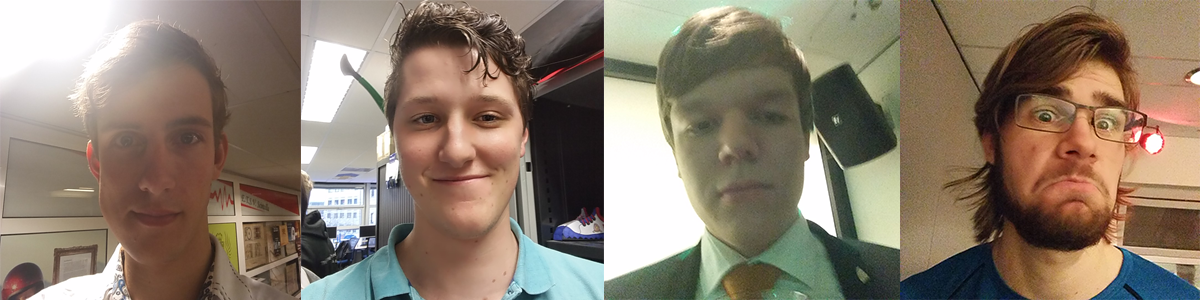
\includegraphics[scale=0.2]{pictures}
	\caption{Example pictures taken by subjects}
	\label{fig:pictures}
\end{figure}

Since only the actual face, and not the background of the picture, is of interest to this research, the pictures were normalized. Facial recognition/identification systems will also normalize pictures; therefore this is not regarded as part of the process nor as a contribution to the computation time the provided method in this research will require. Because of the limited scope of this research, thus the pictures where normalized manually using Adobe Photoshop CC 2015. Examples of the normalized pictures in figure \ref{fig:pictures} are shown in figure \ref{fig:normalized}. The normalization was done by boxing the face of one subject and taking that as the first normalized image. The distance between the eyes of that subject was then measured and used to normalize the remaining pictures, keeping the size of the box equal to the one of the first subject and the distance between the eyes equal to the distance between the eyes of the first subject.

\begin{figure}[h]
	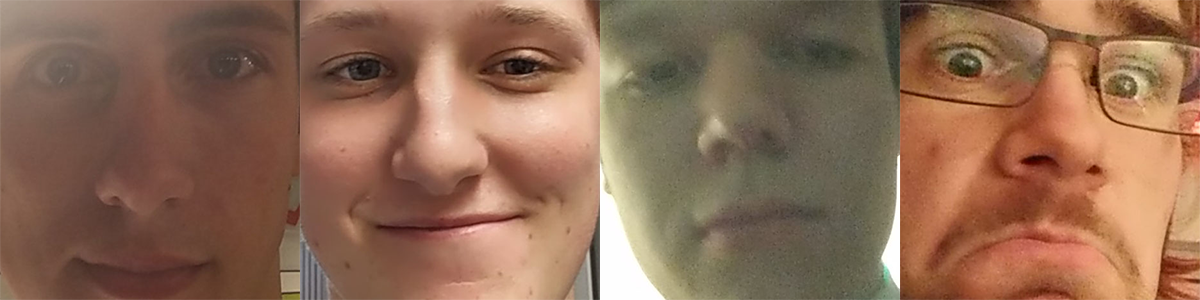
\includegraphics[scale=0.2]{normalized}
	\caption{Normalized versions of figure \ref{fig:pictures}}
	\label{fig:normalized}
\end{figure}


\subsection{Image analysis algorithm} \label{lbp}
The method in this research implements a micro-texture analysis based method called Local Binary Patterns (LBP). The LBP-algorithm consists of the following steps:
\begin{enumerate}
	\item Split the image up into cells
	\item For each pixel in the cell, compare its value to the value of its surrounding neighbours.
	\item If the neighbours value is higher, register a zero, otherwise register a one. This results in an 8-digit binary number.
	\item Compute the histogram over the cell of the frequency of occurrence of each binary number.
	\item Concatenate the histograms of each of the cells of the image.
\end{enumerate}

The LBP-algorithm in this research splits the images up into four cells over which it calculates the histograms. An example for LBP-algorithm over a single pixel is given in figure \ref{fig:lbp_pixel}. An example histogram of one cell is given in figure \ref{fig:histogram} and an example of concatenated histograms is shown in figure \ref{fig:concat_histograms}.

\begin{figure}[h]
	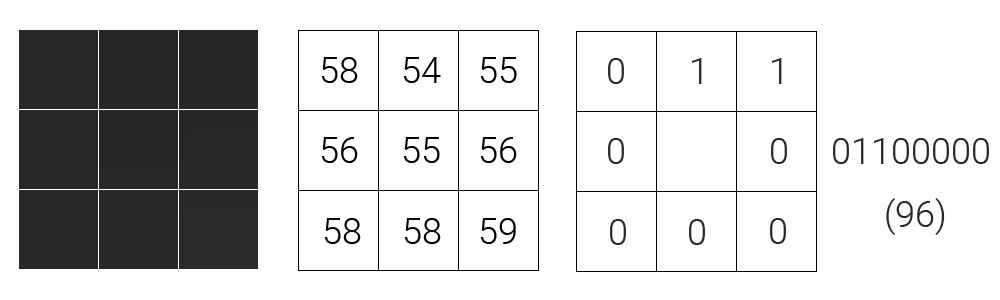
\includegraphics[scale=0.2]{lbp_pixel}
	\caption{Steps 2 and 3 of the LBP-algorithm}
	\label{fig:lbp_pixel}
\end{figure}

\begin{figure}[h]
	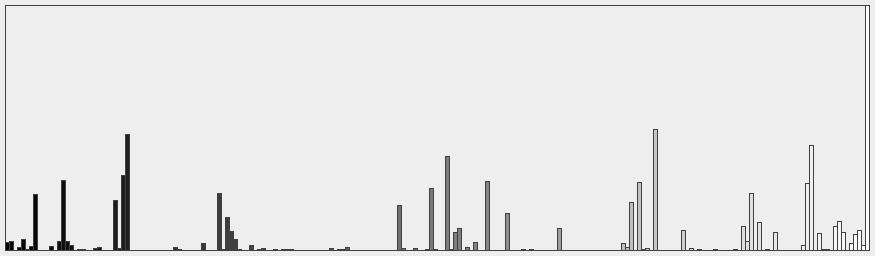
\includegraphics[scale=0.2]{histogram}
	\caption{Step 4  of the LBP-algorithm}
	\label{fig:histogram}
\end{figure}

\begin{figure}[h]
	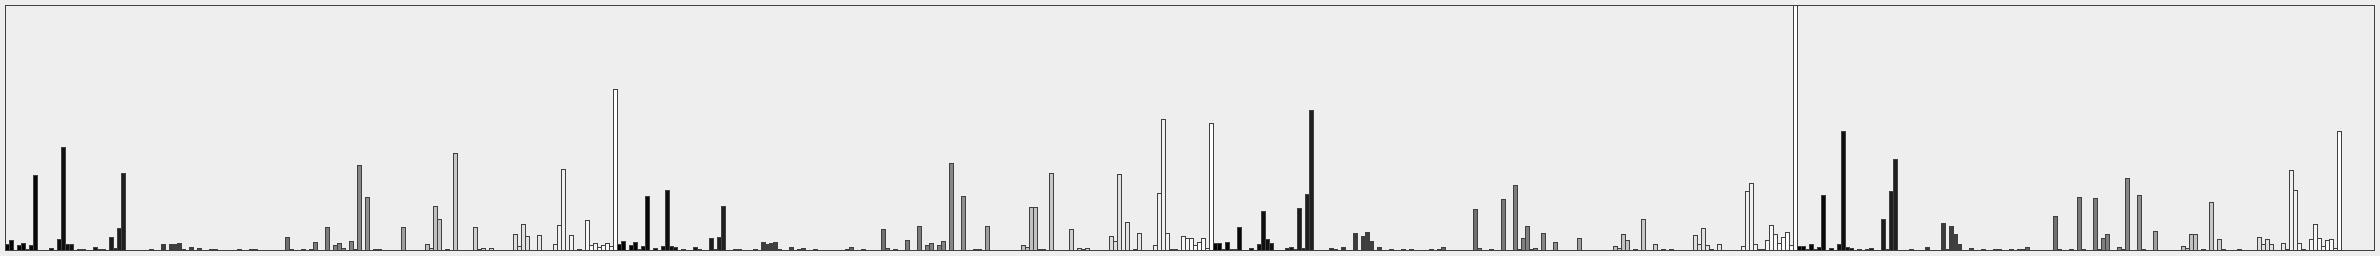
\includegraphics[scale=0.1]{concat_histograms}
	\caption{Step 5 of the LBP-algorithm}
	\label{fig:concat_histograms}
\end{figure}

\subsection{Classification of images}
The histograms calculated per image (see section \ref{lbp}) can be used to classify the images, where we consider two classes: real faces and spoofed faces. This classification is done through machine learning. A certain amount of images (histograms) is labelled with the class they belong to. They are then used to train a support vector machine \cite{hsu2003practical}, a binary linear classifier. This classifier works as follows:

The concatenated histograms of the images are mapped to points in a space. This mapping is done in such a way that the points belong to a certain class are mapped close to another while keeping a maximum distance to the other class. Thus there will be two groups of dots in the space, one group to which the real faces belong and one to which the spoofed faces belong.

Once the classifier has been trained with some real and spoofed faces, it can be used to classify new faces. For such a face (image) we once again compute the concatenated histogram with LBP which we then feed to the classifier. The classifier will map it into the space it trained before and will identify to which group it is situated closest. The classifier can then use the label of that group as the class the analysed face belongs to.

\section{Results} \label{results}

\subsection{Trained model} \label{model}
The dataset consists of twenty faces, twenty paper-recaptures and twenty screen-recaptures resulting in a total of sixty images. To train the classifier, six subjects, a total of eighteen images, were separated from the dataset. The remaining fourteen subjects, forty-two images, were used to generate tests. The model derived from training with six subjects is shown in figure \ref{fig:model}.

\begin{figure}[h]
	
\includegraphics[scale=0.4]{model}
	\caption{The linear binary classifier trained with six subjects}
	\label{fig:model}
\end{figure}

It seems to sufficiently separate the real faces (coloured blue) from the paper and screen faces (coloured yellow).

\subsection{Testing subjects} \label{tests}
However, when the other subjects are plotted in the same way, the results as shown in figure \ref{fig:tests} are found. In figure \ref{fig:tests} the screen faces have been coloured pink to show the clear difference between the two spoofing methods.

\begin{figure}[h]
	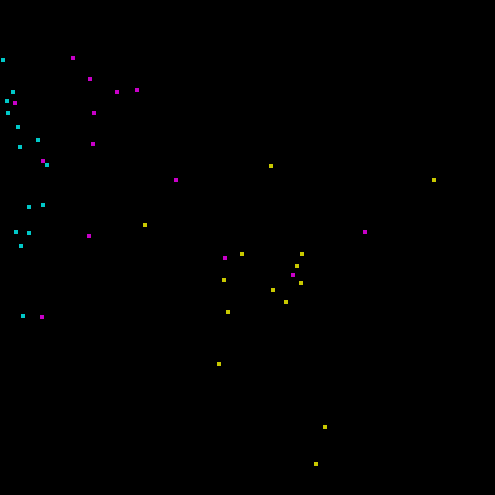
\includegraphics[scale=0.4]{tests}
	\caption{The plotted remaining fourteen test-subjects}
	\label{fig:tests}
\end{figure}

As further ellaborated on in section \ref{stats}, there was only one image that was able to generate a false accept. This image was indeed a screen recapture. Nevertheless, the image is not distinctly different from the other screen recaptures to the human eye \footnote{Not all subjects allowed for their pictures to be published, which is why the false accept image is not shown}.

\subsection{Answering research questions} \label{stats}
Fourteen subjects were tested on the classifier that was trained as explained in \ref{model}. Only one image was able to generate a false accept, and three images were able to generate a false reject. Thus the achieved FAR is 2.4\% and the achieved FRR is 7.1\%.

Besides achieving certain percentages regarding accepts and rejects of images, the processing time of the algorithm is also of importance to this research. The average time of the classification of all forty-two images was measured, where the entire time taken to classify an image was measured. This means both the LBP-algorithm as classification through the binary linear classifier. The average time taken was 67 milliseconds.

\section{Discussion} \label{discussion}
The results of this research are unfortunately limited due to limited time. It requires a rather large amount of manual work and time to construct an elaborate dataset on this matter. Because of the absence of time the used dataset was quite limited. The results found are, however, nonetheless meaningful in this research.

The first sub-question, whether or not a low FAR and low FRR could be achieved, is not entirely answered. The FAR was aimed to be below 2.2\% which unfortunately did not succeed, as the research achieved a FAR of 2.4\% as explained in section \ref{stats}. However, as explained in section \ref{model}, this could well be because of a limited dataset and limited training of the model. The results as shown in section \ref{results} are not conclusive because of the limited dataset. However, it does show that with a small amount of training data, most classification (93.5\%) can be successful. When a larger and more varied dataset is constructed, more accurate results could be determined. In a general sense, a machine learning algorithm, such as the binary linear classifier, will perform better when trained with more data. Thus the results found in this research proof to be at least promising.

The second research question was whether or not the classification of faces could be done in a non-intrusive and relatively fast way. The method discussed in this research is clearly non-intrusive. The user only has to show his/her face to the front-camera of his/her mobile phone.

About the waiting times, the following can be said. The results found in this research were generated on a desktop machine with rather sufficient (graphics accelerated) processing power. The computer took only 67 milliseconds per image to classify it. Mobile phones that are equipped with a front-camera should have sufficient processing power to still have the classification done within reasonable times.

Therefore, both research questions are not fully answered, but the found results are promising.

\bibliographystyle{abbrv}
\bibliography{sigproc}

\balancecolumns
\end{document}
